% -*- root: ../main.tex -*-

\documentclass[../main.tex]{subfiles}
\begin{document}

\chapter{Reduzierte-Basis-Methode} % (fold)
\label{chapter:rbm}

Aufbauend auf das Petrov"=Galerkin"=Verfahren des vorherigen Kapitels führen wir nun die Reduzierte"=Basis"=Methode (kurz RB"=Methode) ein.
Zunächst folgen einige theoretische Grundlagen und Ausführungen zur numerischen Umsetzung dieser Methode, bevor wir mit einigen beispielhaften Anwendungen auf die betrachtete Problemstellung abschließen.

\section{Grundlagen} % (fold)
\label{sub:grb:rb:grundlagen}

Wir beginnen mit einer kurzen Motivation und orientieren uns in diesem Abschnitt an den Arbeiten von \textcite{Rozza2008} sowie \textcite{Patera:2007un}, welche einen weit tieferen Einblick bieten.
Bei der Reduzierte"=Basis"=Methode handelt es sich um ein relativ junges Verfahren, welches vor allem in den letzten zehn Jahren viel Aufmerksamkeit und Weiterentwicklung erfahren hat.

Zunächst wollen wir erneut geeignete Rahmenbedingungen in Form eines abstrakten Variationsproblems schaffen.
Seien dazu zwei Hilberträume $\mathcal X$ und $\mathcal Y$ und eine abgeschlossene, konvexe Parametermenge $\mathcal P \subset \mathbb{R}^{p}$ für ein $p \in \mathbb{N}$ gegeben.
Weiter seien $b \colon \mathcal X \times \mathcal Y \times \mathcal P \to \mathbb{R}$ eine parametrische stetige Bilinearform und $f \colon \mathcal Y \to \mathbb{R}$ ein stetiges lineares Funktional.
Wir betrachten das abstrakte parametrische Variationsproblem:
\begin{equation}
\label{eq:abstraktes_parametrische_vp}
    \text{Sei } \bm \sigma \in \mathcal P, \text{ finde } u(\bm \sigma) \in \mathcal X \text{ mit} \quad b(u(\bm \sigma), v; \bm \sigma) = f(v) \quad \fa v \in \mathcal Y.
\end{equation}

Reduzierte"=Basis"=Methoden bieten sich dann an, wenn das Variationsproblem für einen gegebenen Parameter in Echtzeit oder immer wieder für viele verschiedene Parameter gelöst werden muss.
Um dies mit zufriedenstellender Genauigkeit effizient bewerkstelligen zu können, konzentriert man sich auf die Lösungsmenge
\begin{equation}
\label{eq:stetige_loesungsmenge}
    \mathcal M := \Set{u(\bm \sigma) \in \mathcal X \given \bm \sigma \in \mathcal P}.
\end{equation}
Erfüllt die Bilinearform aus \cref{eq:abstraktes_parametrische_vp} gewisse Regularitätseigenschaften bezüglich des Parameters, dann bildet $\mathcal M$ oftmals eine Mannigfaltigkeit mit vergleichsweise niedriger Dimension.

Um diese Tatsache ausnutzen zu können, müssen wir $\mathcal M$ zunächst durch ein diskretes Analogon ersetzen.
Dazu werden meist Galerkin"=Verfahren verwendet, weswegen wir an dieser Stelle das Petrov"=Galerkin"=Verfahren des vorherigen Kapitels nutzen um eine abstrakte Diskretisierung durchzuführen.
Seien $\mathcal X_{\mathcal N} \subset \mathcal N$ und $\mathcal Y_{\mathcal N} \subset \mathcal Y$ Unterräume der Dimension $\mathcal N \in \mathbb{N}$.
Weiter nehmen wir an, dass diese Diskretisierung für alle $\bm \sigma \in \mathcal P$ zu einem korrekt gestellten Variationsproblem führt, welches gegeben sei durch:
\begin{equation}
\label{eq:diskretes_abstraktes_parametrisches_vp}
    \text{Sei } \bm \sigma \in \mathcal P, \text{ finde } u_{\mathcal N}(\bm \sigma) \in \mathcal X_{\mathcal N} \text{ mit} \quad b(u_{\mathcal N}(\bm \sigma), v; \bm \sigma) = f(v) \quad \fa v \in \mathcal Y_{\mathcal N}.
\end{equation}
Da die RB"=Methode maßgeblich auf diese Petrov"=Galerkin"=Diskretisierung und nicht das eigentliche Variationsproblem \cref{eq:abstraktes_parametrische_vp} aufbaut, werden wir \cref{eq:diskretes_abstraktes_parametrisches_vp} mit dem Präfix \emph{Truth} kenntlich machen.
Die Truth"=Lösungsmenge sei nun definiert als
\begin{equation}
\label{eq:truth_loesungsmenge}
    \mathcal M_{\mathcal N} := \Set{u_{\mathcal N}(\bm \sigma) \in \mathcal X_{\mathcal N} \given \bm \sigma \in \mathcal P}.
\end{equation}
Dies erlaubt die Konstruktion eines niedrigdimensionalen Unterraums $\mathcal X_{N} \subset \mathcal M_{\mathcal N} \subset \mathcal X_{\mathcal N}$, welcher als Ansatzraum eines weiteren Galerkin"=Verfahrens dienen wird.
Dies ist die Grundidee der RB"=Methoden.
\cref{figure:rbm_loesungsmenge} veranschaulicht dies skizzenhaft.

\begin{figure}[tb]
    \centering
    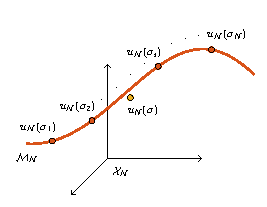
\includegraphics[width=0.6\textwidth]{figures/rb.pdf}
    \caption[%
    Skizze zur Motivation der Reduzierte-Basis-Methode.
    ]{
        Beispiel der Funktionsweise der Reduzierte"=Basis"=Methode im Falle eines eindimensionalen Parameters $\sigma$.
        Die Reduzierte"=Basis"=Lösungen $u_{N}(\sigma)$ ergeben sich als Linearkombinationen der Truth"=Lösungen $u_{\mathcal N}(\sigma_{i})$ für gewisse $\sigma_{i} \in \mathcal P$.
        }
    \label{figure:rbm_loesungsmenge}
\end{figure}

Die Konstruktion des niedrigdimensionalen Ansatzraumes $\mathcal X_{N}$ erfolgt unter dem Aspekt, den durch das zweite Galerkin"=Verfahren zusätzlich eingeführten Fehler für alle Parameter des Parameterraums $\mathcal P$ zu minimieren, was in einem hohen Rechenaufwand resultiert.
Dies motiviert die bei RB"=Methoden übliche Zerlegung in ein zwei Stufen.
Die erste Stufe, die sogenannte \emph{Offline-Phase}, dient dazu den Ansatzraum $\mathcal X_{N}$ unter dem genannten Gesichtspunkt zu konstruieren und muss nur einmal ausgeführt werden.
In der zweiten Stufe, der \emph{Online-Phase}, kann dieses niedrigdimensionale System verwendet werden, um Lösungen für gegebene Parameter auszuwerten und eine garantierte Fehlerschranke zu berechnen.
Da im Allgemeinen $N \ll \mathcal N$ gilt, wird hierbei als weiteres Ziel die Unabhängigkeit der Berechnungen in der Online-Phase von der Dimension $\mathcal N$ verfolgt.

Weiter führt diese Zerlegung zu einem wichtigen Kriterium für respektive gegen die Anwendung der RB"=Methode, da der benötigte Aufwand für die Offline-Phase meist erst ab einer hohen Anzahl an zu bestimmenden Lösungen in der Online-Phase amortisiert wird.

Wir widmen uns nun den formalen Grundlagen der RB"=Methode und beginnen mit einer grundlegenden Definition.

\begin{Definition}
\label{definition:rb_variationsproblem}
    Es seien $N \in \mathbb{N}$ und $\mathcal S_{N} := \Set{ \bm \sigma_{i} \given i = 1, \dots, N } \subset \mathcal P$ die sogenannte \emph{Sample-Menge}.
    Wir bezeichnen die Truth-Lösungen $u_{\mathcal N}(\bm \sigma_{i})$ als \emph{Snapshots} und definieren den RB"=Ansatzraum $\mathcal X_{N}$ als
    \begin{equation}
        \mathcal X_{N} := \spn \Set{ u_{\mathcal N}(\bm \sigma_{i}) \given i = 1, \dots, N} = \spn \Set{ \phi_{i} \given i = 1, \dots, N},
    \end{equation}
    wobei $\Phi_{N} := \Set{ \phi_{i} \given i = 1, \dots, N}$ eine geeignete Orthonormalbasis ist, sowie einen $N$-dimensionalen Unterraum  $\mathcal Y_{N} \subset \mathcal Y_{\mathcal N}$.
    Als RB"=Variationsproblem von \cref{eq:diskretes_abstraktes_parametrisches_vp} bezeichnen wir das  Variationsproblem:
    \begin{equation}
    \label{eq:rb_abstraktes_parametriches_vp}
        \text{Sei } \bm \sigma \in \mathcal P, \text{ finde } u_{N}(\bm \sigma) \in \mathcal X_{N} \text{ mit} \quad b(u_{N}(\bm \sigma), v; \bm \sigma) = f(v) \quad \fa v \in \mathcal Y_{N}.
    \end{equation}
    Fernen nennen wir $u_{N}(\bm \sigma)$ \emph{Reduzierte"=Basis"=Lösung}.
\end{Definition}

Um die notationelle Wiederholung gering zu halten, seien für den Rest dieses Abschnitts stets durch $u_{N}(\bm \sigma) \in \mathcal X_{N}$ die Reduzierte-Basis-Lösung und durch $u_{\mathcal N}(\bm \sigma) \in \mathcal X_{\mathcal N}$ die Truth-Lösung zu einem Parameter $\bm \sigma \in \mathcal P$ gegeben.

Wie zuvor bei den Petrov"=Galerkin"=Verfahren muss auch bei \cref{eq:rb_abstraktes_parametriches_vp} sichergestellt werden, dass es sich dabei um ein korrekt gestelltes Problem handelt.
Wir werden später sehen, dass diese Eigenschaft bei geschickter Wahl des Testraumes $\mathcal Y_{N}$ vom Truth"=Variationsproblem vererbt wird, und nehmen deswegen an dieser Stelle an, dass dies stets erfüllt ist.

Da es sich bei der RB"=Diskretisierung ebenfalls um ein Galerkin"=Verfahren handelt, erhalten wir Analoga der Aussagen \cref{satz:galerkin_stabilitaet} sowie \cref{satz:lemma_von_cea}, welche hier nicht wiederholt werden, wobei die Truth-Räume $\mathcal X_{\mathcal N}$ und $\mathcal Y_{\mathcal N}$ die Rolle der Hilberträume $\mathcal X$ und $\mathcal Y$ einnehmen.

Weiter soll an dieser Stelle angemerkt werden, warum wir eine Galerkin"=Diskretisierung \cref{eq:diskretes_abstraktes_parametrisches_vp} als Grundlage und nicht das eigentliche Variationsproblem \cref{eq:abstraktes_parametrische_vp} verwenden.
Neben dem offensichtlichen Grund, der Berechenbarkeit der Lösung, ist die zugrundeliegende Prämisse die Folgende:
Nach \cref{satz:lemma_von_cea} kann mit der Petrov"=Galerkin"=Lösung $u_{\mathcal N}(\bm \sigma)$ die exakte Lösung $u(\bm \sigma)$ unter gewissen Annahmen beliebig gut approximiert werden.
Betrachten wir weiter die einfache Abschätzung
\begin{equation}
    \norm{u(\bm \sigma) - u_{N}(\bm \sigma)}_{\mathcal X} \leq \norm{u(\bm \sigma) - u_{\mathcal N}(\bm \sigma)}_{\mathcal X} + \norm{u_{\mathcal N}(\bm \sigma) - u_{N}(\bm \sigma)}_{\mathcal X},
\end{equation}
dann entspricht dies gerade der Tatsache, das der erste Summand beliebig klein gehalten werden kann.
Dies erlaubt uns, lediglich den Fehler zwischen Truth- und RB"=Lösung zu berücksichtigen, und führt weiter zu folgender Definition.

\begin{Definition}\label{definition:rbm_fehler_und_residuum}
    Als \emph{Fehler} $e_{N}(\bm \sigma) \in \mathcal X_{\mathcal N}$ bezeichnen wir $e_{N}(\bm \sigma) := u_{\mathcal N}(\bm \sigma) - u_{N}(\bm \sigma)$.
    Weiter definieren wir das \emph{Residuum} $r_{N}(\blank; \bm \sigma) \colon \mathcal Y_{\mathcal N} \to \mathbb{R}$ als
    \begin{equation}\label{eq:variationsproblem_residuum}
        r_{N}(v; \bm \sigma) := b(e_{N}(\bm \sigma), v; \bm \sigma), \quad v \in \mathcal Y_{\mathcal N}.
    \end{equation}
\end{Definition}

\begin{Lemma}\label{lemma:rbm_residuum_ist_funktional}
    Das Residuum $r_{N}(\blank; \bm \sigma)$ ist für alle $\bm \sigma \in \mathcal P$ ein stetiges lineares Funktional, kurz also $r_{N}(\blank; \bm \sigma) \in \mathcal Y_{\mathcal N}'$.

    \begin{Beweis}
        Sowohl Linearität als auch Stetigkeit sind direkt ersichtlich, denn nach Definition erhalten wir
        \begin{equation}
            \begin{aligned}
            r_{N}(v; \bm \sigma)
            &= b(e_{N}(\bm \sigma), v; \bm \sigma)
            = b(u_{\mathcal N}(\bm \sigma), v; \bm \sigma) - b(u_{N}(\bm \sigma), v; \bm \sigma)
            \\&= f(v) - b(u_{N}(\bm \sigma), v; \bm \sigma)
            \end{aligned}
        \end{equation}
        und diese Eigenschaften damit von $f$ und $b$.
    \end{Beweis}
\end{Lemma}

Das Residuum kann nun verwendet werden, um eines der wichtigsten Konstrukte der RB-Methoden zu definieren.

\begin{Lemma}\label{lemma:rbm_fehler_schranke}
    Sei $\beta_{\mathrm{LB}}(\bm \sigma) > 0$ eine untere Schranke für $\beta_{\mathcal N}(\bm \sigma)$.
    Dann gilt
    \begin{equation}
        \norm{u_{\mathcal N}(\bm \sigma) - u_{N}(\bm \sigma)}_{\mathcal X} \leq \Delta_{N}(\bm \sigma) := \frac{\norm{r_{N}(\blank; \bm \sigma)}_{\mathcal Y_{\mathcal N}'}}{\beta_{\mathrm{LB}}(\bm \sigma)},
    \end{equation}
    wobei wir $\Delta_{N}(\bm \sigma)$ als \emph{a posteriori-Fehlerschätzer} bezeichnen.

    \begin{Beweis}
        Wir können \cref{eq:variationsproblem_residuum} als Variationsproblem \cref{eq:diskretes_abstraktes_parametrisches_vp} auffassen, welches unter den getroffenen Annahmen die eindeutige Lösung $e_{N}(\bm \sigma)$ besitzt.
        Die Abschätzung folgt nun aus \cref{satz:galerkin_stabilitaet}.
    \end{Beweis}
\end{Lemma}

Dieser a posteriori-Fehlerschätzer bildet das Herzstück der RB"=Methode, da mit ihm in der Offline-Phase eine möglichst optimale Wahl der Parameter-Samples erreicht werden kann, während er in der Online-Phase zur Berechnung einer garantierten Fehlerschranke zwischen Truth- und RB-Lösung verwendet wird.
Dazu setzt man weiter woraus, dass die untere Schranke $\beta_{\mathrm{LB}}(\bm \sigma)$ berechenbar ist.
Wir werden bei der nachfolgenden numerischen Umsetzung darauf eingehen, wie dies bewerkstelligt werden kann.

Bevor wir uns dieser widmen, wollen wir an dieser Stelle noch ein Maß für die Güte des Fehlerschätzers einführen.

\begin{Lemma}
\label{lemma:effektivitaet}
    Die \emph{Effektivität} $\eta_{N}(\bm \sigma)$ des a posteriori-Fehlerschätzers ist beschränkt durch
    \begin{equation}
        1 \leq \eta_{N}(\bm \sigma) := \frac{\Delta_{N}(\bm \sigma)}{\norm{u_{\mathcal N}(\bm \sigma) - u_{N}(\bm \sigma)}_{\mathcal X}} \leq \frac{\gamma_{\mathcal N}(\bm \sigma)}{\beta_{\mathrm{LB}}(\bm \sigma)},
    \end{equation}
    wobei $\gamma_{\mathcal N}(\bm \sigma)$ die Stetigkeitskonstante der Bilinearform $\restr{b(\blank, \blank; \bm \sigma)}{\mathcal X_{\mathcal N} \times \mathcal Y_{\mathcal N}}$ sei.

    \begin{Beweis}
        Die Abschätzung nach unten ergibt sich direkt aus \cref{lemma:rbm_fehler_schranke}.
        Sei nun $\bm \sigma \in \mathcal P$ beliebig.
        Eine Anwendung des Rieszschen Darstellungssatz liefert für $r_{N}(\blank; \bm \sigma)$ ein $\hat{e}_{N} \in \mathcal Y_{\mathcal N}$ mit $r_{N}(v; \bm \sigma) = \skp{\hat{e}_{N}}{v}{\mathcal Y}$ für alle $v \in \mathcal Y_{\mathcal N}$ und $\norm{r_{N}(\blank; \bm \sigma)}_{\mathcal Y_{\mathcal N}'} = \norm{\hat{e}_{N}}_{\mathcal Y}$.
        Mit der Stetigkeit der Bilinearform erhalten wir damit die Abschätzung
        \begin{equation}
            \norm{\hat{e}_{N}}_{\mathcal Y}^{2}
            = \skp{\hat{e}_{N}}{\hat{e}_{N}}{\mathcal Y}
            = r_{N}(\hat{e}_{N}; \bm \sigma)
            = b(e_{N}(\bm \sigma), \hat{e}_{N}; \bm \sigma)
            \leq \gamma_{\mathcal N}(\bm \sigma) \norm{e_{N}(\bm \sigma)}_{\mathcal X} \norm{\hat{e}_{N}}_{\mathcal Y},
        \end{equation}
        oder kurz
        \begin{equation}
            \norm{\hat{e}_{N}}_{\mathcal Y} \leq \gamma_{\mathcal N}(\bm \sigma) \norm{e_{N}(\bm \sigma)}_{\mathcal X}.
        \end{equation}
        Zusammen mit der Definition des a posteriori-Fehlerschätzers $\Delta_{N}(\bm \sigma)$ liefert dies nun
        \begin{equation}
            \eta_{N}(\bm \sigma)
            = \frac{\Delta_{N}(\bm \sigma)}{\norm{u_{\mathcal N}(\bm \sigma) - u_{N}(\bm \sigma)}_{\mathcal X}}
            \leq \frac{\gamma_{\mathcal N}(\bm \sigma) \norm{e_{N}(\bm \sigma)}_{\mathcal X}}{\beta_{\mathrm{LB}}(\bm \sigma)\norm{u_{\mathcal N}(\bm \sigma) - u_{N}(\bm \sigma)}_{\mathcal X}}
            = \frac{\gamma_{\mathcal N}(\bm \sigma)}{\beta_{\mathrm{LB}}(\bm \sigma)}.
        \end{equation}
    \end{Beweis}
\end{Lemma}

Dieses Ergebnis ist wichtig, denn es garantiert, dass der a posteriori-Fehlerschätzer weder zu pessimistisch noch zu optimistisch ist.
Insbesondere garantiert es, dass der tatsächliche Fehler durch den a posteriori-Fehlerschätzer stets korrekt nach oben abgeschätzt wird.

% TODO: noch etwas zur Konvergenz sagen?

\section{Numerische Umsetzung} % (fold)
\label{sub:grb:rb:numerische_umsetzung}

Wir richten unser Augenmerk nun auf die numerische Umsetzung der RB"=Methode und führen an den entsprechenden Stellen weitere, hierfür benötigte Grundlagen ein.
Im Rahmen dieser Arbeit beschränken wir uns auf die Betrachtung parametrische-affiner Variationsprobleme, so wie sie in \cref{lemma:bilinearform_affin_parametrisch} bereits erwähnt wurden, führen sie an dieser Stelle noch einmal in allgemeinerer Form ein.

\begin{Definition}
\label{definition:parametrisch_affine_bf_fuer_rbm}
    Wir nennen eine parametrische Bilinearform $b \colon \mathcal X \times \mathcal Y \times \mathcal P \to \mathbb{R}$ \emph{parametrisch affin}, wenn sie die Form
    \begin{equation}
        b(u, v; \bm \sigma) = \sum_{q = 1}^{Q_{b}} \theta_{q}^{b}(\bm \sigma) b_{q}(u, v), \quad \text{für } u \in \mathcal X, v \in \mathcal Y, \bm \sigma \in \mathcal P,
    \end{equation}
    hat, wobei für $q = 1, \dots, Q_{b}$ durch $\theta_{q}^{b} \colon \mathcal P \to \mathbb{R}$ Abbildungen und durch $b_{q} \colon \mathcal X \times \mathcal Y \to \mathbb{R}$ parameterunabhängige Bilinearformen gegeben seien.
\end{Definition}

Weiter abstrahieren wir an dieser Stelle die Notationen aus \cref{section:galerkin_numerische_umsetzung}.
Die diskreten Räume $\mathcal X_{\mathcal N}$ und $\mathcal Y_{\mathcal N}$ fassen wir als Span entsprechender Basisfunktionen auf und schreiben
\begin{equation}
    \mathcal X_{\mathcal N} = \spn \Set{ \phi_{i} \given i = 1, \dots, \mathcal N },
    \quad
    \mathcal Y_{\mathcal N} = \spn \Set{ \psi_{j} \given j = 1, \dots, \mathcal N }.
\end{equation}
Ebenso schreiben wir die Reduzierte"=Basis"=Räume $\mathcal X_{N}$ und $\mathcal Y_{N}$ als Span der Form
\begin{equation}
    \mathcal X_{N} = \spn \Set{ \zeta_{i} \given i = 1, \dots, N},
    \quad
    \mathcal Y_{N} = \spn \Set{ \eta_{j} \given j = 1, \dots, N},
\end{equation}
wobei $\zeta_{i} \in \mathcal X_{\mathcal N}$ und $\eta_{j} \in \mathcal Y_{\mathcal N}$ für $i, j = 1, \dots, N$ Basisfunktionen seien.
Die zur Bestimmung der Petrov"=Galerkin"=Lösung verwendeten Strukturen schreiben wir ferner als
\begin{equation}
    \begin{aligned}
        \mat{X} &= \left[ \skp{\phi_{i}}{\phi_{j}}{\mathcal X} \right]_{i,j = 1, \dots, \mathcal N},
        &\qquad
        \mat{Y} &= \left[ \skp{\psi_{i}}{\psi_{j}}{\mathcal Y} \right]_{i,j = 1, \dots, \mathcal N},
        \\
        \vec{f} &= \left[ f(\psi_{j}) \right]_{j = 1, \dots, \mathcal N},
        &\qquad
        \mat{B}_{q} &= \left[ b_{q}(\phi_{i}, \psi_{j}) \right]_{j,i = 1, \dots, \mathcal N}, \quad q = 1, \dots, Q_{b}.
    \end{aligned}
\end{equation}

Zunächst wollen wir eine einfaches Verfahren angeben, mit dem wir aus den zugrundeliegenden Petrov"=Galerkin"=Strukturen die für die RB"=Methode benötigten berechnen können.

\begin{Definition}
    Als \emph{Reduzierte"=Basis"=Ansatzfunktion} $u_{N} \in \mathcal X_{N}$ respektive \emph{Testfunktion} $v_{N} \in \mathcal Y_{N}$ bezeichnen wir
    \begin{equation}
        u_{N} := \sum_{i = 1}^{N} u_{N i} \zeta_{i},
        \quad
        v_{N} := \sum_{j = 1}^{N} v_{N j} \eta_{j},
    \end{equation}
    mit den Koeffizientenvektoren $\vec{u}_{N} := [u_{Ni}]_{i = 1, \dots, N} \in \mathbb{R}^{N}$ und $\vec{v}_{N} := [v_{Nj}]_{j = 1, \dots, N} \in \mathbb{R}^{N}$.
\end{Definition}

Schreiben wir für $i,j = 1, \dots, N$ die Koeffizientenvektoren der Basisfunktionen $\zeta_{i} \in \mathcal X_{N}$ und $\eta_{j} \in \mathcal Y_{N}$ bezüglich der Basen von $\mathcal X_{\mathcal N}$ und $\mathcal Y_{\mathcal N}$  als $\bm \zeta_{i}, \bm \eta_{j} \in \mathbb{R}^{\mathcal N}$, dann können wir ferner die Matrizen
\begin{equation}
  \mat{Z} := [\bm \zeta_{i}]_{i = 1, \dots, N} \in \mathbb{R}^{\mathcal N \times N}, \quad \mat{H} := [\bm \eta_{i}]_{i = 1, \dots, N} \in \mathbb{R}^{\mathcal N \times N}
\end{equation}
definieren.
Mit Hilfe dieser beiden Matrizen definieren wir nun die Reduzierte"=Basis"=Matrizen $\mat{B}_{N, q} \in \mathbb{R}^{N \times N}$, $q = 1, \dots, Q_{b}$, und den Reduzierte"=Basis"=Lastvektor $\vec{f}_{N} \in \mathbb{R}^{N}$ definieren via
\begin{equation}
    \begin{aligned}
        \mat{B}_{N,q} &:= \left[ b_{q}(\zeta_{i}, \eta_{j}) \right]_{j, i = 1, \dots, N} = \mat{H}\tran \mat{B}_{q} \mat{Z}, \quad q = 1, \dots, Q_{b}, \\
        \vec{f}_{N} &:= \left[ f(\eta_{j}) \right]_{j = 1, \dots, N} = \mat{H}\tran \vec{f}
    \end{aligned}
\end{equation}
und analog auch die entsprechenden Norminduzierenden Matrizen $\mat{X}_{N}, \mat{Y}_{N} \in \mathbb{R}^{N \times N}$ durch
\begin{equation}
    \begin{aligned}
    \mat{X}_{N} &:= \left[ \skp{\zeta_{i}}{\zeta_{j}}{\mathcal X} \right]_{i,j = 1, \dots, N} = \mat{Z}\tran \mat{X} \mat{Z}, \\
    \mat{Y}_{N} &:= \left[ \skp{\eta_{i}}{\eta_{j}}{\mathcal Y} \right]_{i,j = 1, \dots, N} = \mat{H}\tran \mat{Y} \mat{H}.
    \end{aligned}
\end{equation}

Um nun die RB"=Lösung $u_{N}(\bm \sigma)$ zu einem Parameter $\bm \sigma \in \mathcal P$ zu bestimmen, reicht es, das lineare Gleichungssystem
\begin{equation}
\label{eq:rbm_gleichungssystem}
    \mat{B}_{N}(\bm \sigma) \vec{u}_{N}(\bm \sigma) = \vec{f}_{N}
\end{equation}
zu lösen, wobei
\begin{equation}
\label{eq:affine_rbm_systemmatrix}
    \mat{B}_{N}(\bm \sigma) = \sum_{q = 1}^{Q_b} \theta_{q}^{b}(\bm \sigma) \mat{B}_{N, q}
\end{equation}
die Systemmatrix und $\vec{u}_{N}(\bm \sigma)$ der Koeffizientenvektor der Lösung ist.

\subsection{Zerlegung in Offline- und Online-Phase} % (fold)
\label{sub:zerlegung_in_offline_und_online_phase}

Wir gehen nun detailliert auf die beiden Phasen der Reduzierte"=Basis"=Methode ein und beginnen mit der einfacheren Online-Phase, bevor wir zur aufwendigeren Offline-Phase übergehen.

\subsubsection{Online-Phase} % (fold)
\label{ssub:online_phase}

In der Online-Phase muss zu einem gegebenen Parameter $\bm \sigma \in \mathcal P$ lediglich die Systemmatrix $\mat{B}_{N}(\bm \sigma)$ anhand der parametrisch-affinen Darstellung \cref{eq:affine_rbm_systemmatrix} berechnet werden, um anschließend die RB"=Lösung $u_{N}(\bm \sigma)$ über das Gleichungssystem \cref{eq:rbm_gleichungssystem} bestimmen zu können.

Ferner bestimmen wir den a posteriori-Fehlerschätzer $\Delta_{N}(\bm \sigma)$ zur Zertifizierung des Fehlers.

% subsubsection online_phase (end)

\subsubsection{Offline-Phase} % (fold)
\label{ssub:offline_phase}

Ziel der Offline-Phase ist die Bestimmung der für die Online-Phase benötigten Strukturen unter dem Gesichtspunkt den maximalen Fehler möglichst zu minimieren.
Dies wird oft auf Basis heuristisch motivierter Strategien getan, da die theoretisch optimale Auswahl der Snapshot-Parameter numerisch nicht umsetzbar ist.
Weiterführend findet man hierzu bei \cite{??} eine umfassende Einführung in die sogenannten \emph{Kolmogorow-N-Weiten}.

Als praktisch umsetzbare Verfahren erfreuen vor allem \emph{Greedy}-Strategien und auf die \emph{Proper Orthogonal Decomposition} aufbauende Algorithmen großer Beliebtheit.
Da wir uns auf einen Greedy-Ansatz beschränken werden, sei zu letzterem an dieser Stelle \cite{} als weitereführende Literatur erwähnt.

Der hier zum Einsatz kommende Ansatz ist unter dem Namen \emph{Greedy Sampling Scheme} bekannt, und lässt sich wie folgt zusammenfassen.
Iterativ wird der Parameter $\bm \sigma^{*} \in \mathcal P$ bestimmt, welcher in der aktuellen reduzierten Basis den Fehler $\norm{e_{N}(\bm \sigma)}_{\mathcal X}$ maximiert.
Durch Hinzunahme der zugehörigen Truth"=Lösung $u_{\mathcal N}(\bm \sigma^{*})$ zur reduzierten Basis erreichen wir somit in jedem Schritt eine maximale Fehlerreduktion.
Da die Auswertung des exakten Fehlers $\norm{e_{N}(\bm \sigma)}_{\mathcal X}$ einen zu hohen Aufwand mit sich liefert, kommt hier der a posteriori-Fehlerschätzer $\Delta_{N}(\bm \sigma)$ aus \cref{lemma:rbm_fehler_schranke} zum Einsatz.
Das daraus resultierende Verfahren findet sich formal genauer in \cref{algorithm:greedy_training}.

Ein offenbar kritischer Punkt des Algorithmus ist die Auswertung des a posteriori-Fehlerschätzers.
Diese setzt sich zum einen aus der Berechnung der Norm des Residuums und aus der Bestimmung einer Schranke für die inf-sup-Konstante.
Wir gehen zunächst auf das einfacher zu handhabende Residuum ein.

\paragraph{Berechnung der Norm des Residuums.} % (fold)
\label{par:berechnung_der_norm_des_residuum}

Um diese zu bestimmen, greifen wir erneut auf den Rieszschen Darstellungssatz zurück und erhalten damit für jedes $\bm \sigma \in \mathcal P$ ein $\hat{e}_{N}(\bm \sigma) \in \mathcal Y_{\mathcal N}$ mit
\begin{equation}
    \norm{\hat{e}_{N}(\bm \sigma)}_{\mathcal Y} = \norm{r_{N}(\blank; \bm \sigma)}_{\mathcal Y_{\mathcal N}'}, \qquad
    r_{N}(v; \bm \sigma) = \skp{\hat{e}_{N}(\bm \sigma)}{v}{\mathcal Y_{\mathcal N}}, \quad \fa v \in \mathcal Y.
\end{equation}
Aufgrund der Definition des Residuums \cref{eq:variationsproblem_residuum} und der parametrisch-affinen Darstellung \cref{definition:parametrisch_affine_bf_fuer_rbm} der Bilinearform $b$ können wir dies verwursten zu
\begin{equation}
    \skp{\hat{e}_{N}(\bm \sigma)}{v}{\mathcal Y}
    = r_{N}(v; \bm \sigma)
    % = f(v) - \sum_{q = 1}^{Q_b} \theta_{q}^{b}(\bm \sigma) b_{q}(u_{N}(\bm \sigma), v)
    = f(v) - \sum_{q = 1}^{Q_b} \sum_{n = 1}^{N} \theta_{q}^{b}(\bm \sigma) u^{(n)}_{N}(\bm \sigma) b_{q}(\zeta_{n}, v).
\end{equation}
Fassen wir nun weiter die Abbildungen $b_{q}(\zeta_{n}, \blank) \colon \mathcal Y_{\mathcal N} \to \mathbb{R}$ als Funktionale auf, dann sind diese stetig und linear und wir können erneut den Rieszschen Darstellungssatz anwenden.
Dies liefert die Existenz von $\hat{f}, \hat{b}^{n}_{q} \in \mathcal Y_{\mathcal N}$, $n = 1, \dots, N,$, $q = 1, \dots, Q_b$, mit
\begin{equation}
    \begin{aligned}
        f(v) &= \skp{\hat{f}}{v}{\mathcal Y}, \quad \fa v \in \mathcal Y_{\mathcal N},
        \\
        b_{q}(\zeta_{n}, v) &= \skp{\hat{b}^{n}_{q}}{v}{\mathcal Y_{\mathcal N}}, \quad \fa v \in \mathcal \mathcal Y_{\mathcal N}.
    \end{aligned}
\end{equation}
Zusammen mit obiger Darstellung erhalten wir damit
\begin{equation}
    \hat{r}_{N}(\bm \sigma) = \hat{f} - \sum_{q = 1}^{Q_b} \sum_{n = 1}^{N} \theta_{q}^{b}(\bm \sigma) u_{N}^{(n)}(\bm \sigma) \hat{b}^{n}_{q}.
\end{equation}
Die Norm des Residuums kann damit über
\begin{equation}
    \begin{aligned}
        \norm{\hat{r}_{N}(\bm \sigma)}_{\mathcal Y}^{2}
        &= \skp{\hat{r}_{N}(\bm \sigma)}{\hat{r}_{N}(\bm \sigma)}{\mathcal Y}
        \\&= \begin{multlined}[t]
            \skp{\hat{f}}{\hat{f}}{\mathcal Y}
                - 2 \sum_{q = 1}^{Q_b} \sum_{n = 1}^{N} \theta_{q}^{b}(\bm \sigma) u_{N}^{(n)}(\bm \sigma) \skp{\hat{b}^{n}_{q}}{\hat{f}}{\mathcal Y}
                \\+ \sum_{q, p = 1}^{Q_b} \sum_{n, m = 1}^{N} \theta_{q}^{b}(\bm \sigma) \theta_{p}^{b}(\bm \sigma) u_{N}^{(n)}(\bm \sigma) u_{N}^{(m)}(\bm \sigma) \skp{\hat{b}^{n}_{q}}{\hat{b}^{m}_{p}}{\mathcal Y}.
        \end{multlined}
    \end{aligned}
\end{equation}

Diese Berechnung kann nun effizient in eine Offline- und eine Online-Phase zerlegt werden.

\begin{description}[font=\normalfont\itshape]
    \item[Offline:] Berechne und speichere $\skp{\hat{f}}{\hat{f}}{\mathcal Y}$, $\skp{\hat{b}^{n}_{q}}{\hat{f}}{\mathcal Y}$ und $\skp{\hat{b}^{n}_{q}}{\hat{b}^{m}_{p}}{\mathcal Y}$.
    \item[Online:] Werte obige Darstellung aus.
\end{description}

TODO: Alternative Berechnung über Matrixschreibweise?

% paragraph berechnung_der_norm_des_residuum (end)

\paragraph{Berechnung der unteren Schranke für die inf-sup-Konstante.} % (fold)
\label{par:berechnung_der_unteren_schranke_f_r_die_inf_sup_konstante_}

Da die exakte Bestimmung der inf-sup-Konstante $\beta_{\mathcal N}(\bm \sigma)$ für jeden Parameter $\bm \sigma \in \Xi_{\mathrm{train}}$ laufzeittechnisch nicht vertretbar ist, wird ein Verfahren benötigt, welches auf effiziente Weise eine möglichst genaue untere Schranke $\beta_{\mathrm{LB}}(\bm \sigma)$ liefert.
Hierfür verwenden wir die zu diesem Zweck entwickelte \ac{scm} und orientieren uns an der Originalarbeit von \textcite{Huynh2007}, wobei wir an dieser Stelle nur die Idee des Verfahrens wiederholen wollen.
Weiter wurden bei der Implementierung die Verbesserungen von \textcite{Chen2009} berücksichtigt, die wir aber nicht weiter ausführen werden.

Da die \ac{scm} auf die Berechnung der Koerzivitätskonstante einer symmetrischen parametrischen Bilinearform ausgelegt ist, müssen wir zunächst die nötigen Rahmenbedingungen schaffen.
Wir werden später darauf eingehen, wie wir mit der \ac{scm} die gewünschte inf-sup-Schranke bestimmen können.

Es sei eine abstrakte symmetrische, parametrisch-affine Bilinearform $a \colon \mathcal X \times \mathcal X \times \mathcal P \to \mathbb{R}$ durch
\begin{equation}
    a(u, v; \bm \sigma) = \sum_{q = 1}^{Q_a} \theta_{q}^{a} a_{q}(u, v), \quad u,v \in \mathcal X,
\end{equation}
gegeben, wobei $\theta_{q}^{a} \colon \mathcal P \to \mathbb{R}$ stetige Funktionen und $a_{q} \colon \mathcal X \times \mathcal X \to \mathbb{R}$ symmetrische, stetige und parameterunabhängige Bilinearformen seien.
Wie zuvor sei $\mathcal X_{\mathcal N} \subset \mathcal X$ eine Diskretisierung eines Galerkin"=Verfahrens.
Wir wollen nun eine Schranke $\alpha_{\mathrm{LB}}(\bm \sigma)$ für die \emph{Koerzivitätskonstante} $\alpha_{\mathcal N}(\bm \sigma)$ bestimmen, welche als
\begin{equation}
    \alpha_{\mathcal N}(\bm \sigma) := \inf_{u \in \mathcal X_{\mathcal N}} \frac{a(u, u; \bm \sigma)}{\norm{u}_{\mathcal X}^{2}}
\end{equation}
definiert ist.

Die Idee hinter der \ac{scm} ist nun, die Bestimmung der obigen Koerzivitätskonstante als lineares Programm aufzufassen.
Dazu sei zunächst die tatsächliche zulässige Menge $\mathcal Z$ definiert als
\begin{equation}
    \mathcal Z := \Set[\bigg]{ \vec{z} = (z_{1}, \dots, z_{Q_a}) \in \mathbb{R}^{Q_a} \given \exists u_{z} \in \mathcal X_{\mathcal N} \colon z_{q} = \frac{a_{q}(u_{z}, u_{z})}{\norm{u_{z}}_{\mathcal X}^{2}}, q = 1, \dots, Q_a}.
\end{equation}
Weiter definieren wir die Zielfunktion
\begin{equation}
    \mathcal J \colon \mathbb{R}^{Q_a} \times \mathcal P \to \mathbb{R}, \quad \mathcal J(\vec{z} ;\bm \sigma) := \sum_{q = 1}^{Q_a} \theta_{q}^{a}(\bm \sigma) z_{q}.
\end{equation}
Mit dieser Konstruktion gilt nun $\alpha_{\mathcal N}(\bm \sigma) = \min_{\vec{z} \in \mathcal Z} \mathcal J(\vec{z}; \bm \sigma)$, es handelt sich aber noch nicht um ein lineares Programm.

Hierfür beschränken wir zunächst die einzelnen Variablen $z_{q}$ von oben und unten durch die Wahl von
\begin{equation}
    \alpha_{q}^{-} := \inf_{u \in \mathcal X_{\mathcal{N}}} \frac{a_{q}(u, u)}{\norm{u}^{2}_{\mathcal X}},
    \quad
    \alpha_{q}^{+} := \sup_{u \in \mathcal X_{\mathcal{N}}} \frac{a_{q}(u, u)}{\norm{u}^{2}_{\mathcal X}},
    \qquad \fa q = 1, \dots, Q_a,
\end{equation}
und des Quaders $B_{Q_a} := \prod_{q = 1}^{Q_a} [\alpha^{-}_{q}, \alpha^{+}_{q}] \subset \mathbb{R}^{Q_a}$.

Weiter benötigen wir eine endliche Teilmenge $\Xi_{\mathrm{train}} \subset \mathcal P$ als Trainingsparameter und definieren hier bereits die Notation $\mathcal C_{K} := \Set{ \bm \sigma_{1}, \dots, \bm \sigma_{K} } \subset \mathcal P$ für eine weitere, noch zu konstruierende Parameterteilmenge.
Ferner sei durch $P_{M}(\bm \sigma; E)$ eine Abbildung gegeben, welche für ein $M \in \mathbb{N}_{0}$ und eine Teilmenge $E \subset \mathcal P$ die bezüglich der euklidischen Norm $M$ nächsten Punkte zu $\bm \sigma$ aus $E$ liefert.
Schließlich seien durch $M_{\alpha}, M_{+} \in \mathbb{N}$ die Anzahl der Stabilitätsbedingungen respektive Positivitätsbedingungen festgelegt.

Mit dieser Vorarbeit lassen sich nun eine Untermenge $\mathcal Z_{\mathrm{LB}}(\bm \sigma; \mathcal C_{K}) \subset \mathcal Z$ und eine Obermenge $\mathcal Z_{\mathrm{UB}}(\mathcal C_{K}) \supset \mathcal Z$ durch
\begin{equation}
    \begin{aligned}
        \mathcal Z_{\mathrm{LB}}(\bm \sigma; \mathcal C_{K}) &:=
        \begin{multlined}[t]
        \Set*{\vec{z} \in B_{Q_a} \given
        \textstyle\sum_{q = 1}^{Q_a} \theta_{q}^{a}(\hat{\bm \sigma})z_{q} \geq \alpha_{\mathcal N}(\bm \sigma)~\fa \hat{\bm \sigma} \in P_{M_{\alpha}}(\bm \sigma; \mathcal C_{K})
        }
        \\ \cap
        \Set*{\vec{z} \in B_{Q_a} \given
        \textstyle\sum_{q = 1}^{Q_a} \theta_{q}^{a}(\hat{\bm \sigma}) z_{q} \geq 0~\fa \hat{\bm \sigma} \in P_{M_{+}}(\bm \sigma; \Xi_{\mathrm{train}})
        },
        \end{multlined}\\
        \mathcal Z_{\mathrm{UB}}(\mathcal C_{K}) &:= \Set[\Big]{ \vec{z}^{*}(\bm \sigma_{k}) := \arg \min_{\vec z \in \mathcal Z} \mathcal J(\vec{z}; \bm \sigma_{k}) \given k = 1, \dots, K}.
    \end{aligned}
\end{equation}
Nach Konstruktion handelt es sich dabei um konvexe Polyeder, sodass wir nun die beiden linearen Programme
\begin{equation}
    \alpha_{\mathrm{LB}}(\bm \sigma; \mathcal C_{K}) := \min_{\vec{z} \in \mathcal Z_{\mathrm{LB}}(\bm \sigma; \mathcal C_{K})} \mathcal J(\vec{z}; \bm \sigma),
    \quad
    \alpha_{\mathrm{UB}}(\bm \sigma; \mathcal C_{K}) := \min_{\vec{z} \in \mathcal Z_{\mathrm{UB}}(\mathcal C_{K})} \mathcal J(\vec{z}; \bm \sigma)
\end{equation}
definieren können.
Es lässt sich nachweisen \cite[Proposition 1]{Huynh2007}, dass diese für beliebige $\mathcal C_{K}, M_{\alpha}$ und $M_{+}$ die Abschätzung
\begin{equation}
    \alpha_{\mathrm{LB}}(\bm \sigma; \mathcal C_{K}) \leq \alpha_{\mathcal N}(\bm \sigma) \leq \alpha_{\mathrm{UB}}(\bm \sigma; \mathcal C_{K}), \quad \fa \bm \sigma \in \mathcal P,
\end{equation}
erfüllen.

Es bleibt lediglich die Konstruktion der Teilmengen $\mathcal C_{K} \subset \mathcal P$ zu klären.
Dazu wird erneut ein Greedy-Verfahren eingesetzt, siehe \cref{algorithm:scm_greedy}.
Dieses wird in der Offline-Phase der \ac{scm} ausgeführt, während in der Online-Phase zur Bestimmung der gesuchten Schranke $\alpha_{\mathrm{LB}}(\bm \sigma)$ ein relativ kleines lineares Programm gelöst werden muss.

\begin{algorithm}[tb]
    \DontPrintSemicolon
    \SetKwInOut{Input}{Eingabe}\SetKwInOut{Output}{Ausgabe}
    \SetKwProg{Proc}{Prozedur}{}{}
    %
    \Input{Menge $\Xi_{\mathrm{train}} \subset \mathcal P$ der Trainingsparameter und Fehlertoleranz $\epsilon_{\mathrm{tol}} > 0$}
    \Output{Reduzierte-Basis-Ansatzraum $\mathcal X_{N}$}
    \BlankLine
    Setze $K = 1$, $\mathcal C_{1} = \Set{\bm \sigma_{1}}$ mit zufälligem $\bm \sigma_{1} \in \Xi_{\mathrm{train}}$\;
    \While{$\max_{\bm \sigma \in \Xi_{\mathrm{train}}} [(\alpha_{\mathrm{UB}}(\bm \sigma; \mathcal C_{K}) - \alpha_{\mathrm{LB}}(\bm \sigma; \mathcal C_{K})) / {\alpha_{\mathrm{UB}}(\bm \sigma; \mathcal C_{K})}] > \epsilon_{\mathrm{tol}}$}{
        $\bm \sigma_{K + 1} \leftarrow \arg \max_{\bm \sigma \in \Xi_{\mathrm{train}}} [(\alpha_{\mathrm{UB}}(\bm \sigma; \mathcal C_{K}) - \alpha_{\mathrm{LB}}(\bm \sigma; \mathcal C_{K})) / {\alpha_{\mathrm{UB}}(\bm \sigma; \mathcal C_{K})}]$\;
        $\mathcal C_{K + 1} \leftarrow \mathcal C_{K} \cup \Set{\bm \sigma_{K + 1}}$\;
        $K \leftarrow K + 1$\;
    }
    \caption{Successive Constraint Method}
    \label{algorithm:scm_greedy}
\end{algorithm}

Das selbe Verfahren lässt schlussendlich auch für die Bestimmung einer inf-sup-Konstante verwenden.
Dazu betrachten wir die bekannte Bilinearform $b$ aus \cref{definition:parametrisch_affine_bf_fuer_rbm} und definieren für jedes $q = 1, \dots, Q_{b}$ mittels Rieszschen Darstellungssatzes einen Operator $T_{q} \colon \mathcal X_{\mathcal N} \to \mathcal Y_{\mathcal N}$ mittels
\begin{equation}
    \skp{T_{q} u}{v}{\mathcal Y} = b_{q}(u, v), \quad u \in \mathcal X_{\mathcal N}, v \in \mathcal Y_{\mathcal N},
\end{equation}
sowie den Operator $T(\bm \sigma) \colon \mathcal X_{\mathcal N} \to \mathcal Y_{\mathcal N}$ mittels
\begin{equation}
    T(\bm \sigma) := \sum_{q = 1}^{Q_b} \theta_{q}^{b}(\bm \sigma) T_{q}.
\end{equation}
Analog zu \cref{par:berechnung_der_inf_sup_konstante} geht ab
Es lässt sich zeigen \cite[476]{Huynh2007}, dass für die inf-sup-Konstante $\beta_{\mathcal N}(\bm \sigma)$ nun die Beziehung
\begin{equation}
    (\beta_{\mathcal N}(\bm \sigma))^{2}
    = \left( \inf_{u \in \mathcal X_{\mathcal N}} \sup_{v \in \mathcal Y_{\mathcal N}} \frac{b(u, v; \bm \sigma)}{\norm{u}_{\mathcal X} \norm{v}_{\mathcal Y}} \right)^{2}
    = \inf_{u \in \mathcal X_{\mathcal N}} \frac{\skp{T(\bm \sigma)u}{T(\bm \sigma)u}{\mathcal Y}}{\norm{u}_{\mathcal X}^{2}}
\end{equation}
gilt, wobei $\skp{T(\bm \sigma)\blank}{T(\bm \sigma)\blank}{\mathcal Y} \colon \mathcal X_{\mathcal N} \times \mathcal X_{\mathcal N} \to \mathbb{R}$ eine symmetrische, parametrische, stetige Bilinearform definiert.
Auf diese kann nun die beschriebene \acl{scm} angewandt werden, um die inf-sup-Konstante abzuschätzen.


% paragraph berechnung_der_unteren_schranke_f_r_die_inf_sup_konstante_ (end)

% subsubsection offline_phase (end)

\clearpage

\begin{algorithm}[tb]
    \DontPrintSemicolon
    \SetKwInOut{Input}{Eingabe}\SetKwInOut{Output}{Ausgabe}
    \SetKwProg{Proc}{Prozedur}{}{}
    %
    \Input{Menge $\Xi_{\mathrm{train}} \subset \mathcal P$ der Trainingsparameter und Fehlertoleranz $\epsilon_{\mathrm{tol}} > 0$}
    \Output{Reduzierte-Basis-Ansatzraum $\mathcal X_{N}$ der Dimension $N$}
    \BlankLine
    Setze $N = 0$, $\mathcal P_{0} = \Set{}$, $\Phi_{0} = \Set{}$, $\mathcal X_{0} = \Set{0}$\;
    \While{$\max_{\bm \sigma \in \Xi_{\mathrm{train}}} \Delta_{N}(\bm \sigma) > \epsilon_{\mathrm{tol}}$}{
        $\bm \sigma_{N + 1} \leftarrow \arg \max_{\bm \sigma \in \Xi_{\mathrm{train}}} \Delta_{N}(\bm \sigma)$\;
        $\mathcal P_{N + 1} \leftarrow \mathcal P_{N} \cup \Set{\bm \sigma_{N + 1}}$\;
        $\Phi_{N + 1} \leftarrow \Phi_{N} \cup \Set{u_{\mathcal N}(\bm \sigma_{N + 1})}$\;
        $\mathcal X_{N + 1} \leftarrow \spn \Phi_{N + 1}$\;
        $N \leftarrow N + 1$\;
    }
    %
    \caption{Greedy Training}
    \label{algorithm:greedy_training}
\end{algorithm}


\paragraph{Konstruktion des Testraumes.} % (fold)
\label{par:konstruktion_des_testraumes_}

Wir haben bisher nicht geklärt, wie der Reduzierte"=Basis"=Testraum $\mathcal Y_{N} \subset \mathcal Y_{\mathcal N}$ bestimmt wird.
Hierzu greifen wir erneut auf den Supremizing-Operator aus \cref{definition:supremizing_operator} zurück und definieren damit einen parameterabhängigen Testraum $\mathcal Y_{N}^{\bm \sigma}$ via
\begin{equation}
    \label{eq:rb_testraum_parameterabhaengig}
    \mathcal Y_{N}^{\bm \sigma} := \Set{ T_{\bm \sigma} u_{\mathcal N}(\bm \sigma_{n}) \given n = 1, \dots, N },
\end{equation}
wobei $T_{\bm \sigma}$ der Supremizing-Operator der Bilinearform $b(\blank, \blank; \bm \sigma) \colon \mathcal X_{\mathcal N} \times \mathcal Y_{\mathcal N} \to \mathbb{R}$ ist.
Diese Wahl des Testraumes ist vorteilhaft, wie die folgende Aussage nachweist.

\begin{Satz}
\label{satz:rb_testraum_liefert_korrekt_gestelltes_problem}
    Das RB"=Variationsproblem \cref{eq:rb_abstraktes_parametriches_vp} mit den Räumen $\mathcal X_{N}$ und $\mathcal Y_{N}^{\bm \sigma}$ ist für alle $\bm \sigma \in \mathcal P$ korrekt gestellt.

    \begin{Beweis}
        Wir weisen die Bedingungen des \acl{bnb}s nach, wobei hier nur die inf"=sup"=Bedingung von Interesse ist.
        Nach Annahme gilt für die Truth"=inf"=sup"=Konstante $\beta_{\mathcal N}(\bm \sigma) > 0$.
        Da nach Definition ferner für $u \in \mathcal X_{N}$ auch $T_{\bm \sigma}u \in \mathcal Y_{N}^{\bm \sigma}$ gilt, erhalten wir damit
        \begin{equation}
            \begin{aligned}
                \beta_{N}(\bm \sigma)
                &= \inf_{u \in \mathcal X_{N}} \sup_{v \in \mathcal Y_{N}^{\bm \sigma}} \frac{b(u, v; \bm \sigma)}{\norm{u}_{\mathcal X} \norm{v}_{\mathcal Y}}
                = \inf_{u \in \mathcal X_{N}} \frac{b(u, T_{\bm \sigma}u; \bm \sigma)}{\norm{u}_{\mathcal X} \norm{T_{\bm \sigma} u}_{\mathcal Y}}
                \\&= \inf_{u \in \mathcal X_{N}} \frac{\norm{T_{\bm \sigma}u}_{\mathcal Y}}{\norm{u}_{\mathcal X}}
                \geq \inf_{u \in \mathcal X_{\mathcal N}} \frac{\norm{T_{\bm \sigma}u}_{\mathcal Y}}{\norm{u}_{\mathcal X}}
                \\&= \beta_{\mathcal N}(\bm \sigma) > 0.
            \end{aligned}
        \end{equation}
    \end{Beweis}
\end{Satz}

Da $\mathcal Y_{N}^{\bm \sigma}$ für jeden Parameter neu aufgebaut werden muss, ist auch hierfür eine Zerlegung in Offline- und Online-Phase erwünscht.
Dazu nutzen wir die parametrisch-affine Darstellung der Bilinearform und definieren für jede Bilinearform $b_{q}$, $q = 1, \dots, Q_b$, den zugehörigen Supremizing-Operatoren als $T_{q}$ und es gilt
\begin{equation}
    T_{\bm \sigma} = \sum_{q = 1}^{Q_b} \theta_{q}^{b}(\bm \sigma) T_{q}.
\end{equation}
Die diskrete Darstellung $\mat{T}_{q} \in \mathbb{R}^{\mathcal N \times \mathcal N}$ der Operatoren $T_q$ ist nach Rieszschem Darstellungssatzes durch $\mat{T}_{q} = \mat{Y}^{-1} \mat{B}_{q}$ gegeben.
Dies erlaubt die folgende Zerlegung:

\begin{description}[font=\normalfont\itshape]
    \item[Offline:]Berechne und speichere für jedes $u_{\mathcal N}(\bm \sigma_{n}) \in \mathcal X_{N}$ die Vektoren $\vec{v}_{q}^{n} := \mat{T}_{q} \vec{u}_{\mathcal N}(\bm \sigma_{n}) = \mat{Y}^{-1} \mat{B}_{q} \vec{u}_{\mathcal N}(\bm \sigma_{n})$.
    \item[Online:] Bestimme $\mathcal Y_{N}^{\bm \sigma}$ durch Auswertung von $\mat{T}_{\bm \sigma} \vec{u}_{\mathcal N}(\bm \sigma_{n}) = \sum_{q = 1}^{Q_b} \theta_{q}^{b}(\bm \sigma) \vec{v}_{q}^{n}$.
\end{description}

% paragraph konstruktion_des_testraumes_ (end)

\section{Beispiele} % (fold)
\label{sec:cha5_rbm:beispiele}

% section experimente (end)

\end{document}
